\part{圆幂与根心}
% 相交弦定理





\section{圆幂}
\begin{definition}[圆幂]
    定义$P$点到圆$O$的圆幂为
    $$\text{Pow}_O(P) = OP^2 - R^2,$$
    其中$R$为圆$O$的半径,$OP$为点$P$到圆心的距离。
\end{definition}


% 圆幂定理
\begin{theorem}[圆幂定理]
    假设平面内有一半径为R的圆O,P为平面内任意一点。
    
    (1) $\text{Pow}_O(P)$根据$P$在圆外,圆上或圆内分别取正值、零、负值。

    (2) 若直线$l$经过点$P$,与圆$O$相交于两点$A$和$B$,则
    $$PA \cdot PB = |\text{Pow}_O(P)|$$

    (3) 若$P$在圆外,$PA$与圆相切于点A,则
    $$PA^2 = |\text{Pow}_O(P)|$$
\end{theorem}
\begin{figure}[H]
    \centering
    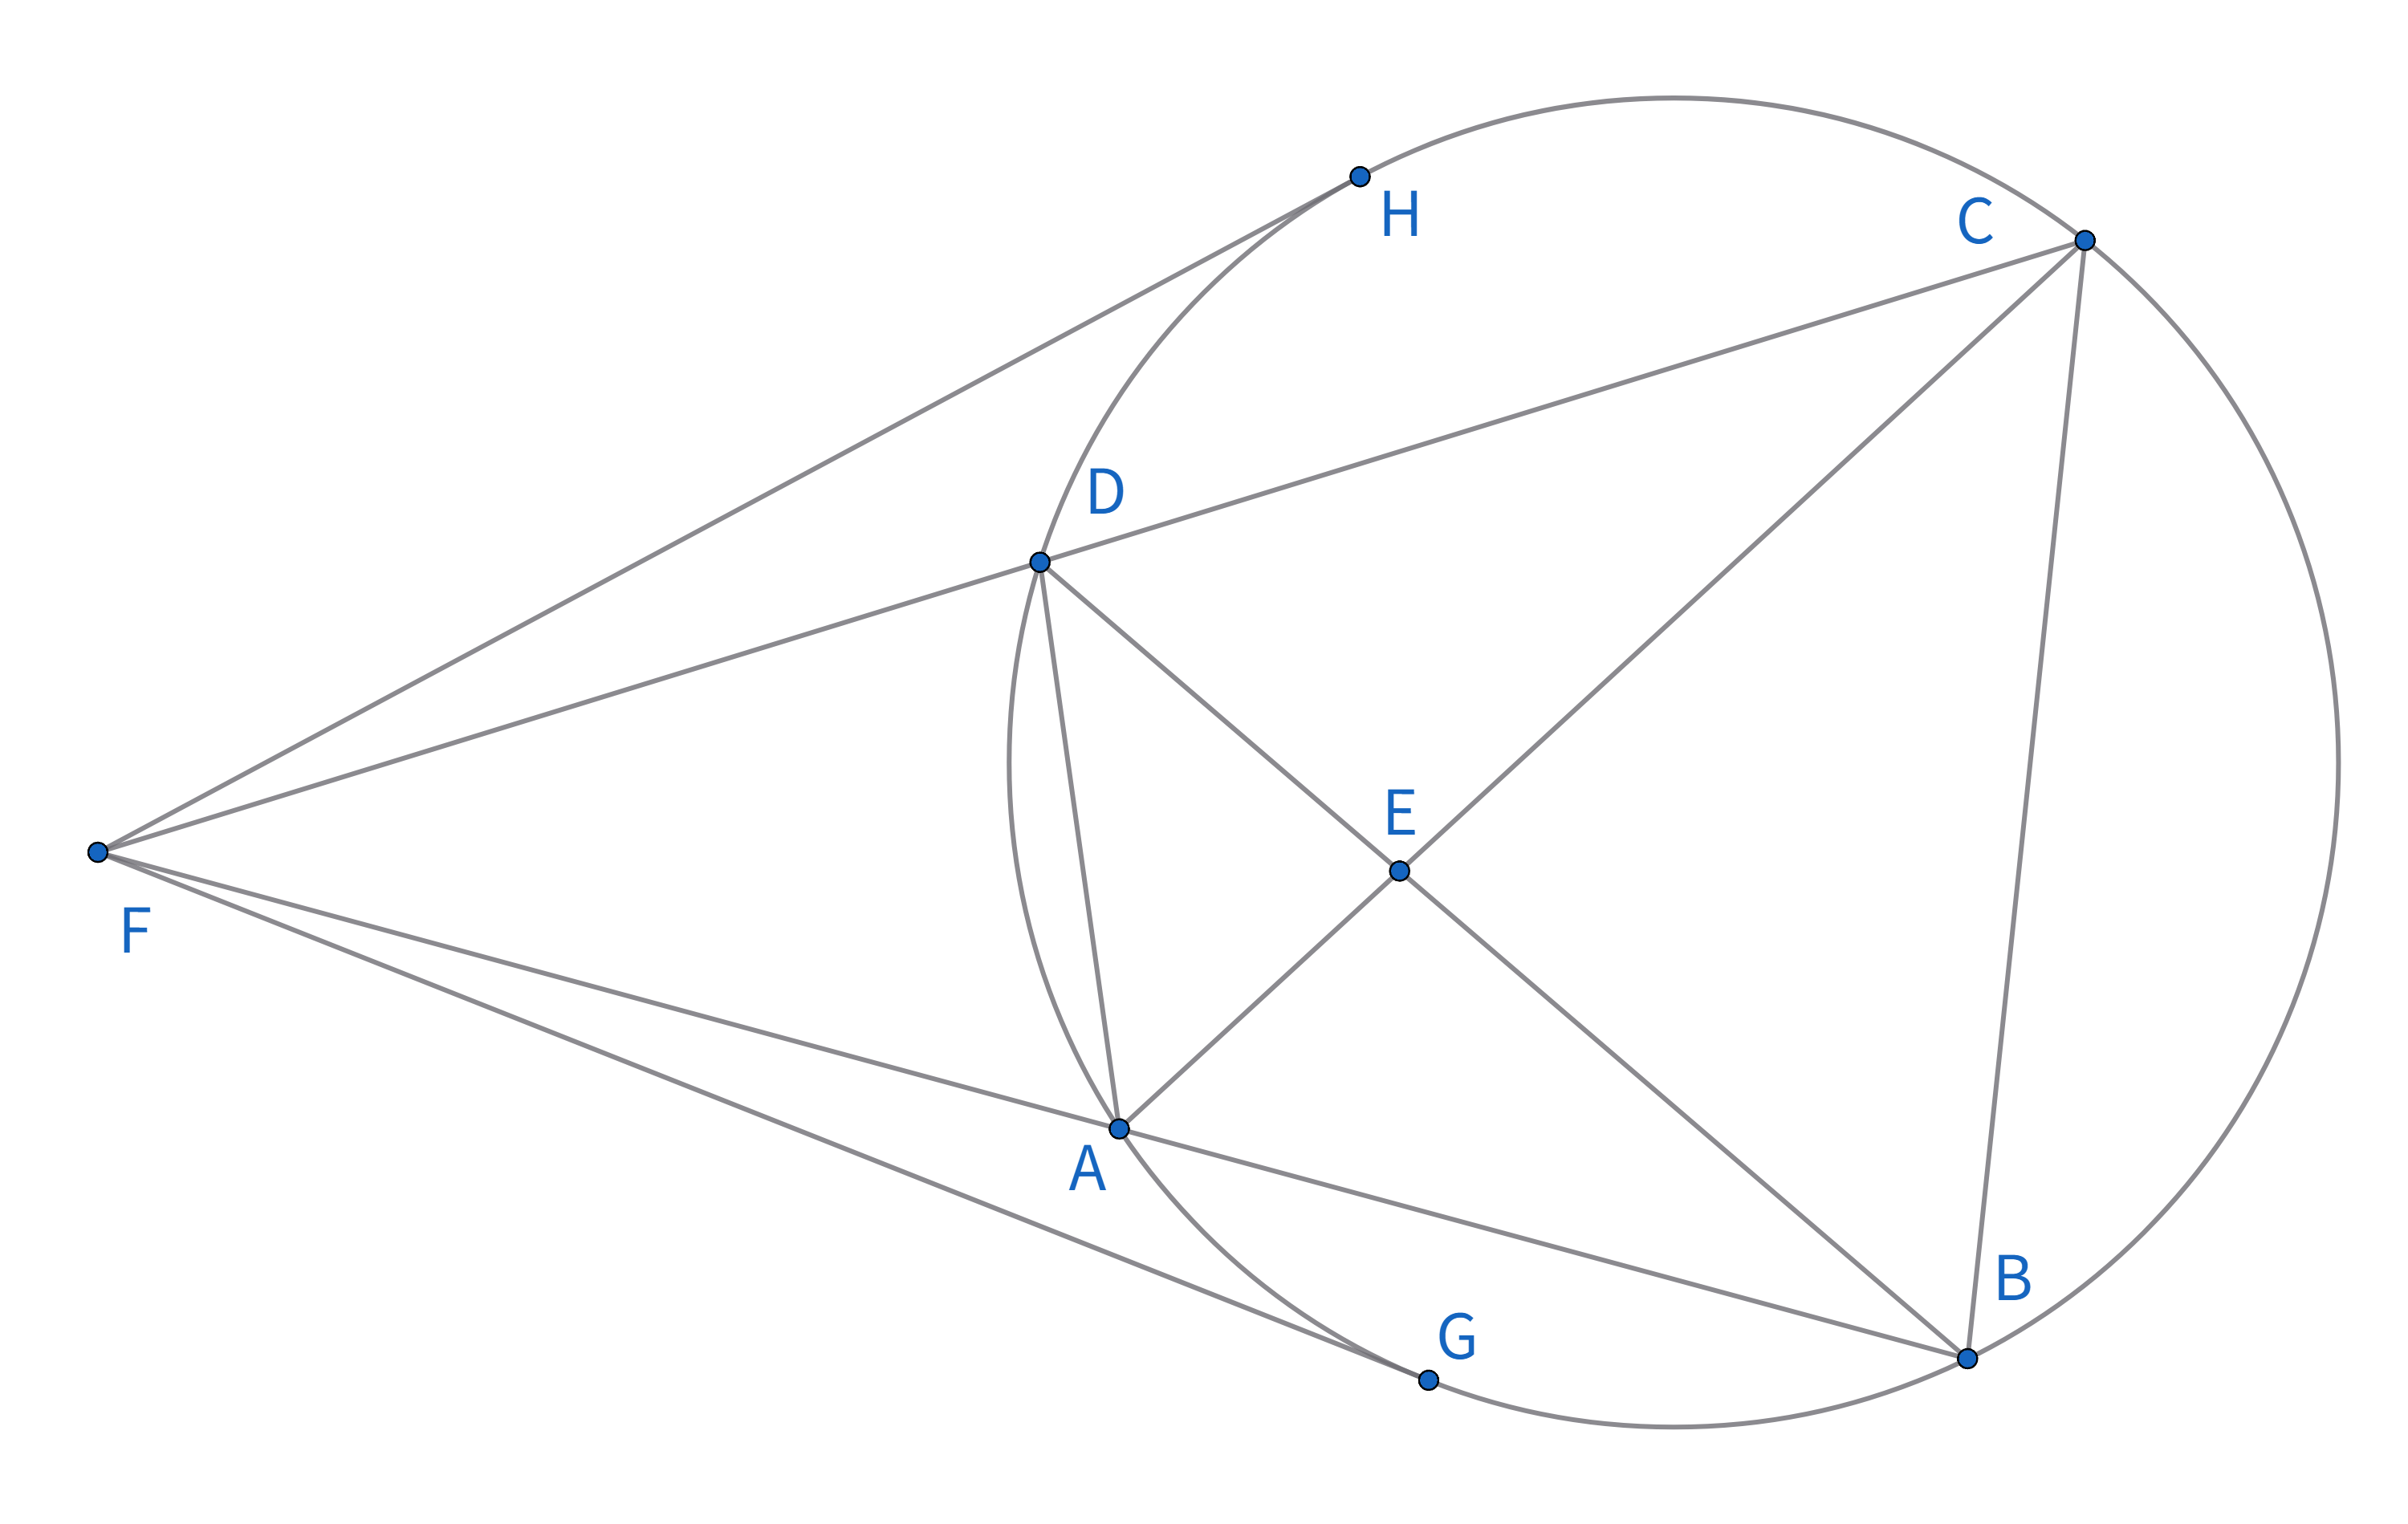
\includegraphics[width=0.7\linewidth]{figures/圆幂定理.png}
    \caption{圆幂定理}
\end{figure}
\begin{remark}
    定点到定圆的圆幂是一个定值,与割线的取法无关。
\end{remark}


\begin{theorem}[圆幂逆定理]
    设 $A, B, C, D$ 是平面上四个不同的点,直线 $AB$ 和 $CD$ 相交于 $P$。假设 $P$ 或者同时在两条线段 $AB$ 和 $CD$ 内,或者同时在两条线段外。若 $PA \cdot PB = PC \cdot PD$,则 $A, B, C, D$ 四点共圆。
\end{theorem}

%-------------------------------------------------------------
\newpage 
\section{根轴}
\begin{theorem}[根轴]
    对于两已知圆有等幂点的轨迹,为一条垂直于连心线的直线。
\end{theorem}
\begin{figure}[H]
    \centering
    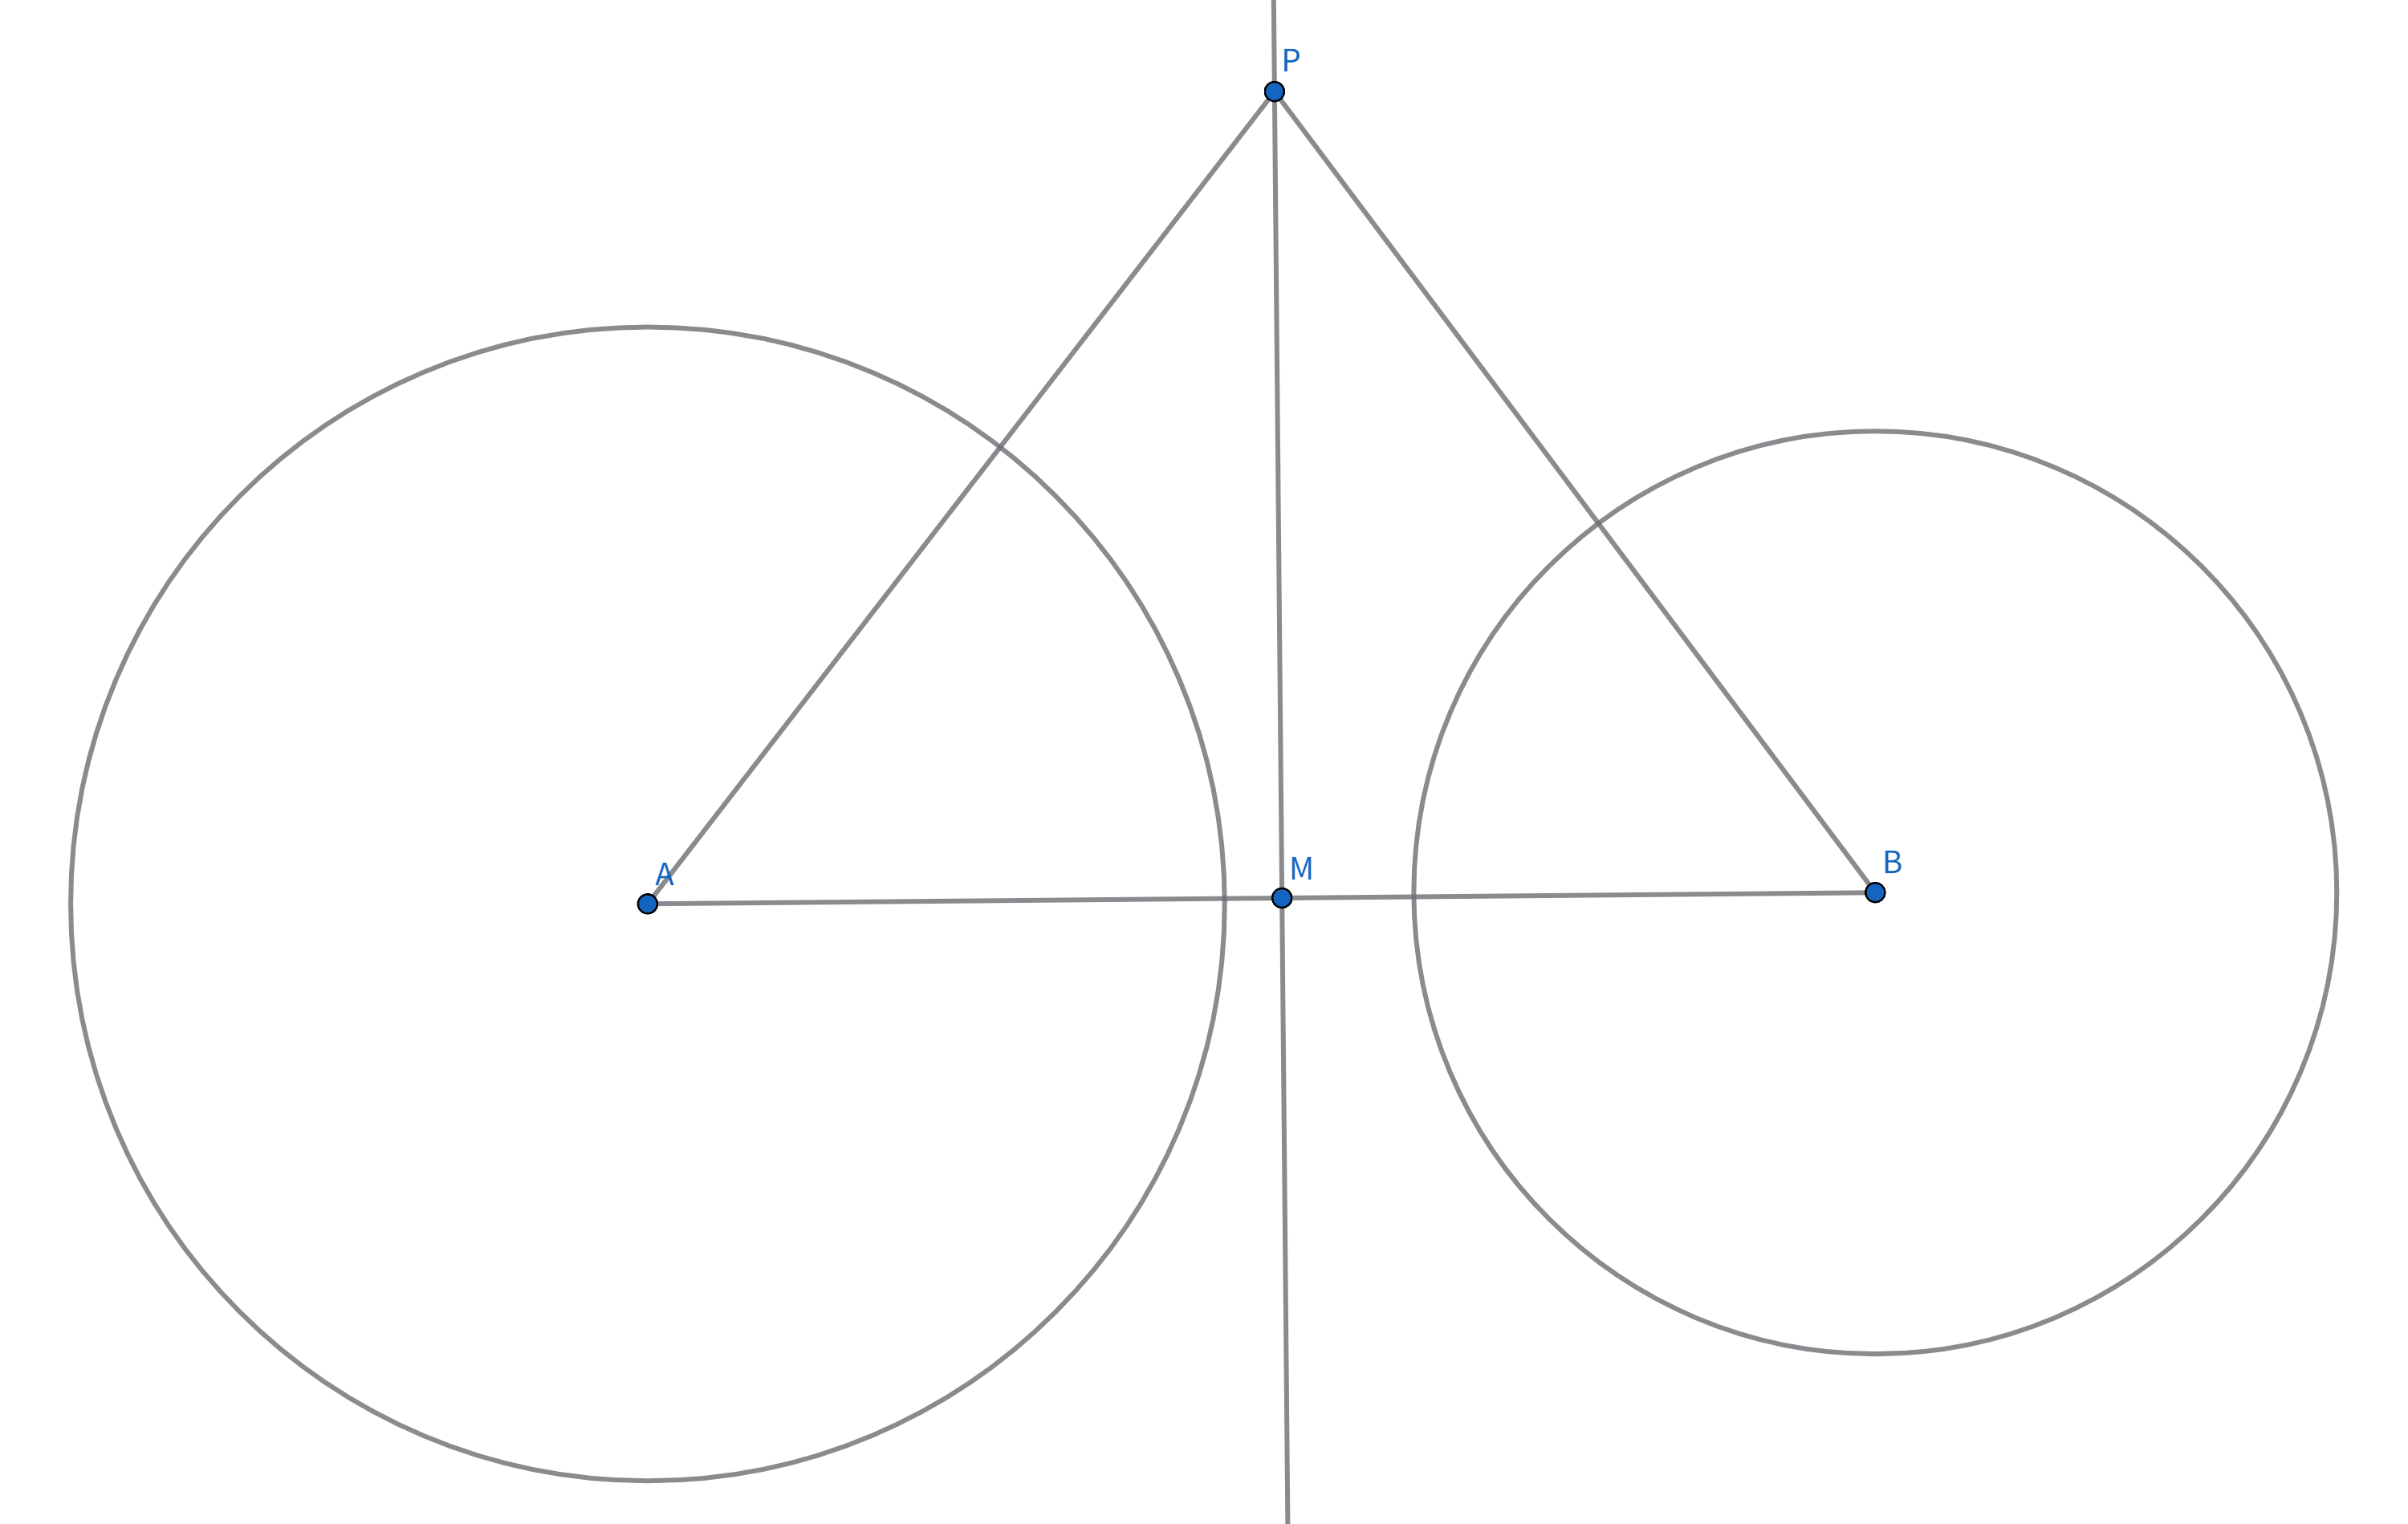
\includegraphics[width=0.7\linewidth]{figures/根轴.png}
    \caption{根轴}
\end{figure}

\begin{proposition}[根轴性质]
    两圆的根轴有如下性质:
    
    (1) 若两圆相交,其根轴就是公共弦所在的直线。
    
    (2) 若两圆相切(内切或外切),其根轴就是过两圆切点的公切线。
    
    (3) 若两圆外离,则两圆的四条公切线的中点在根轴上。
\end{proposition}
\begin{figure}[H]
    \centering
    \hfill % 添加一些水平间距
    \begin{minipage}[t]{0.3\textwidth}
        \centering
        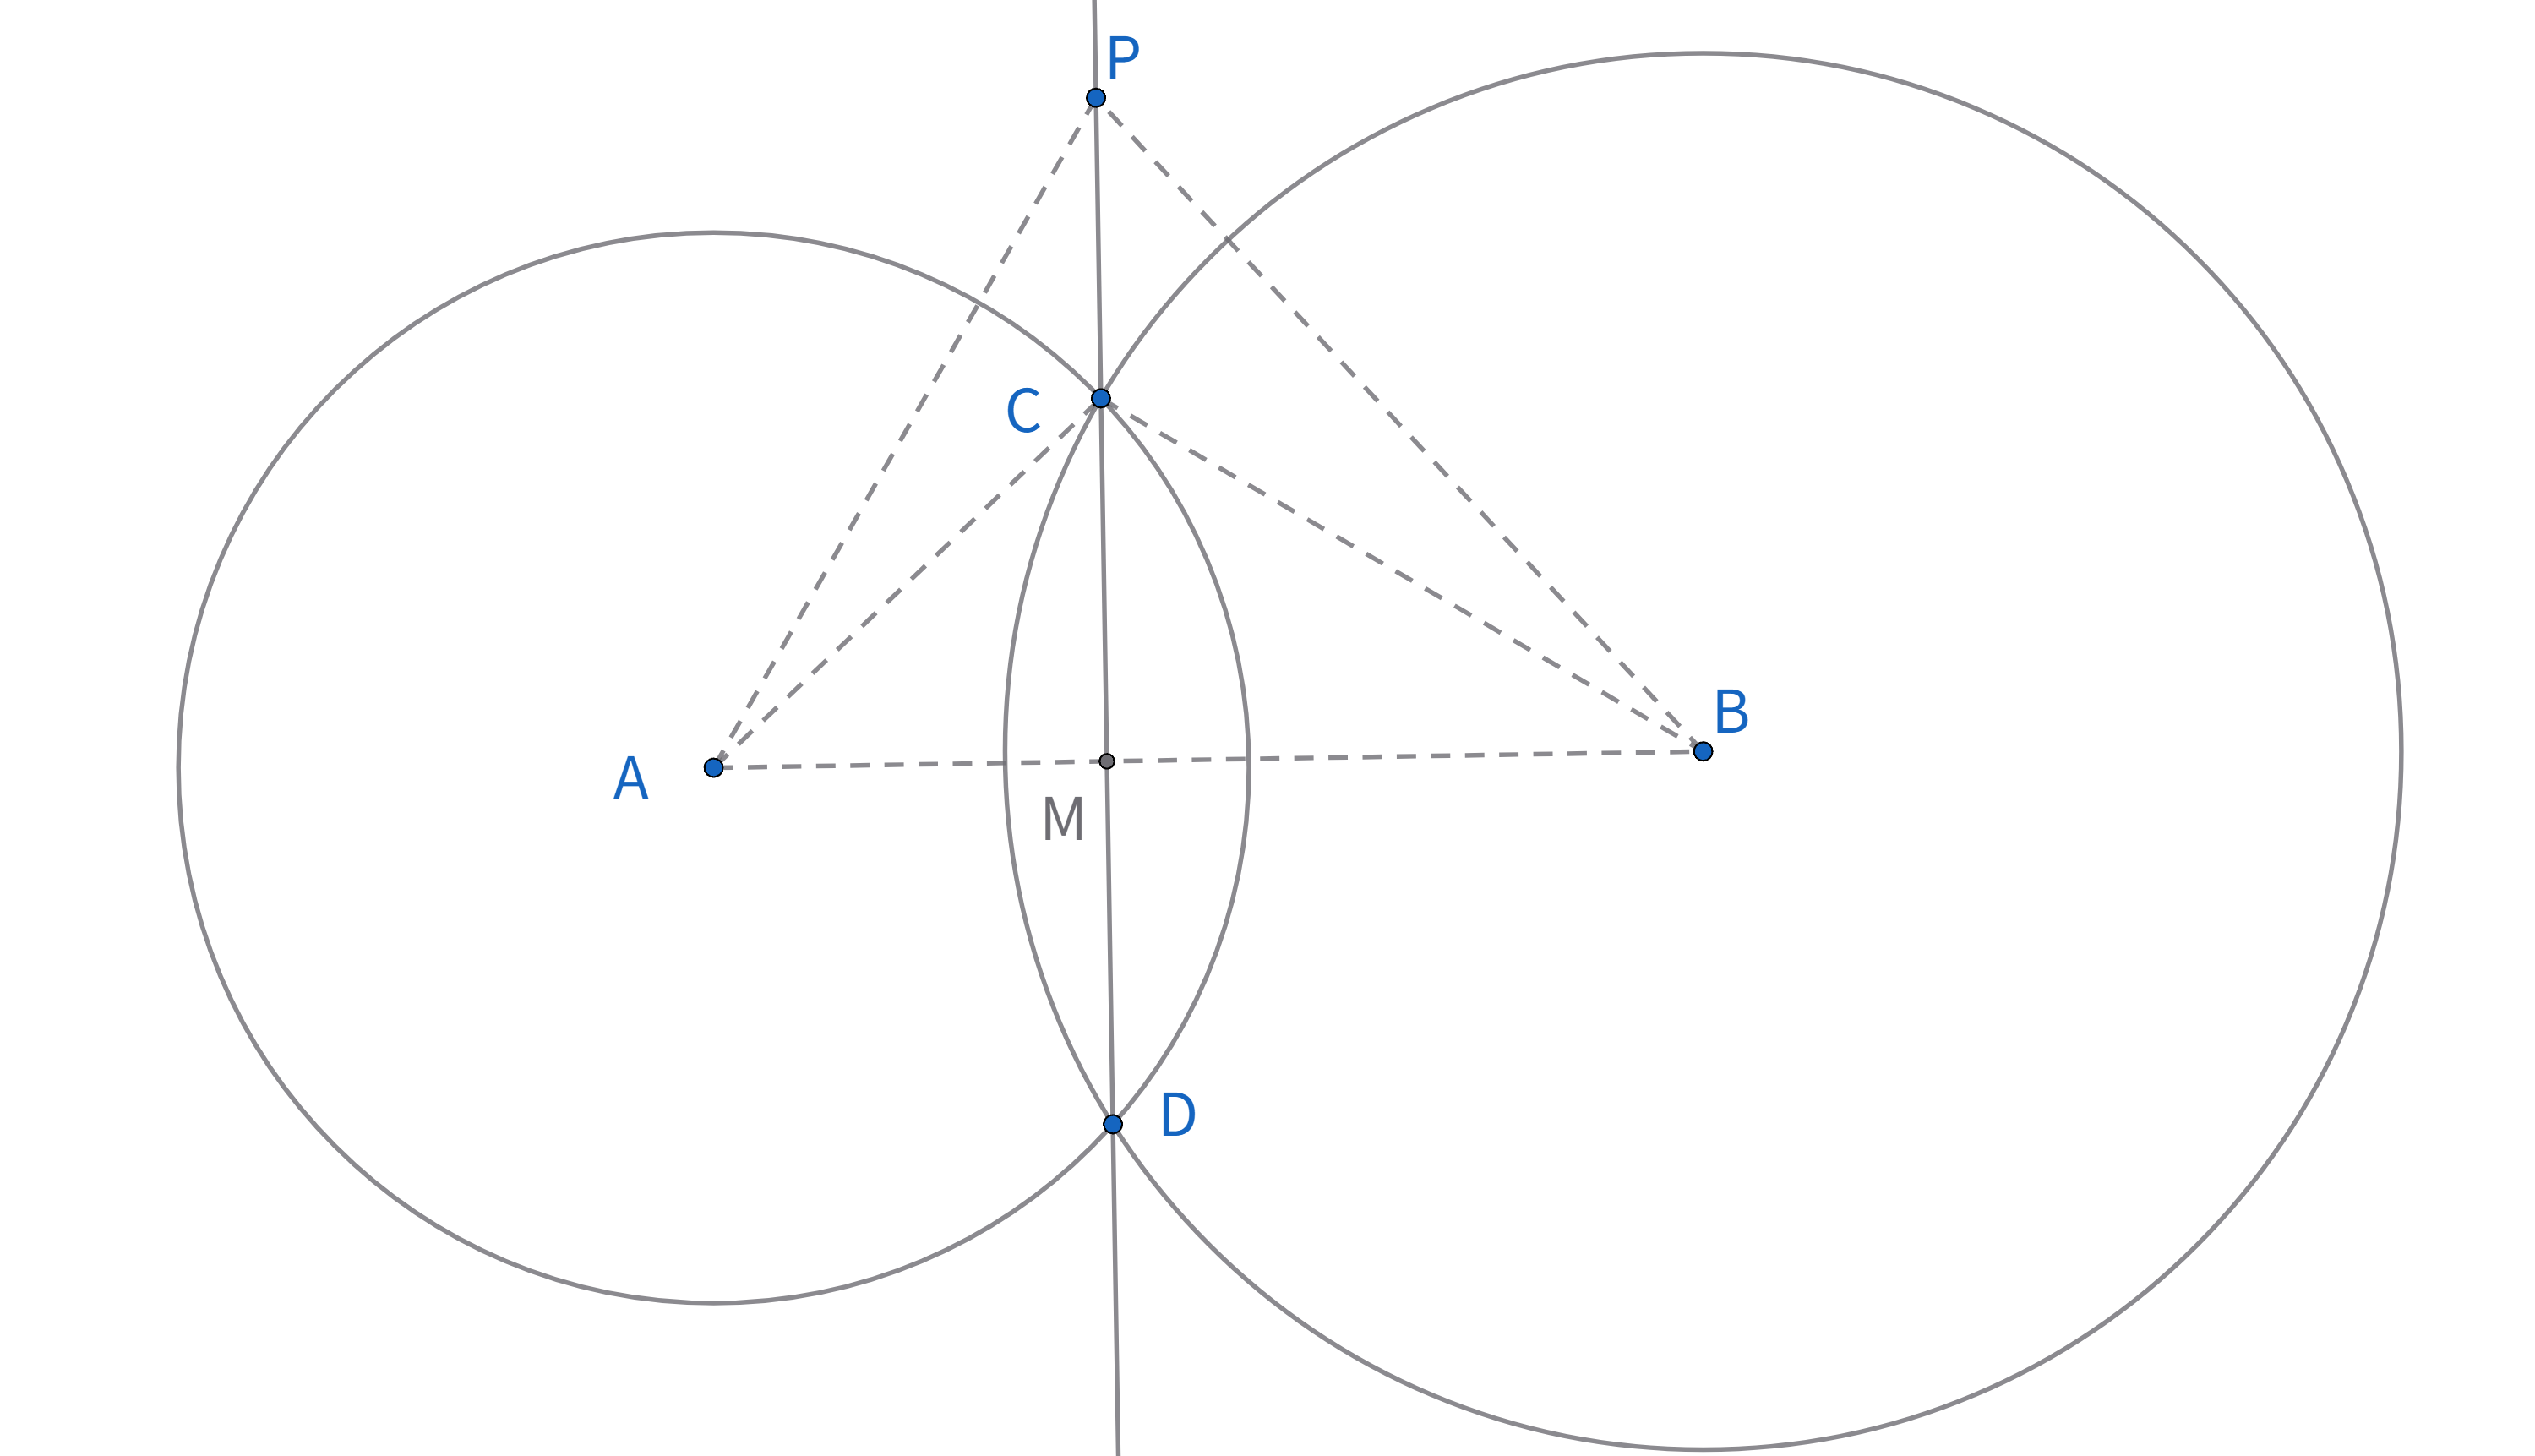
\includegraphics[width=\linewidth]{figures/相交圆根轴.png}
        \caption{相交圆根轴}
    \end{minipage}
    \hfill % 添加一些水平间距
    \begin{minipage}[t]{0.3\textwidth}
    \centering
    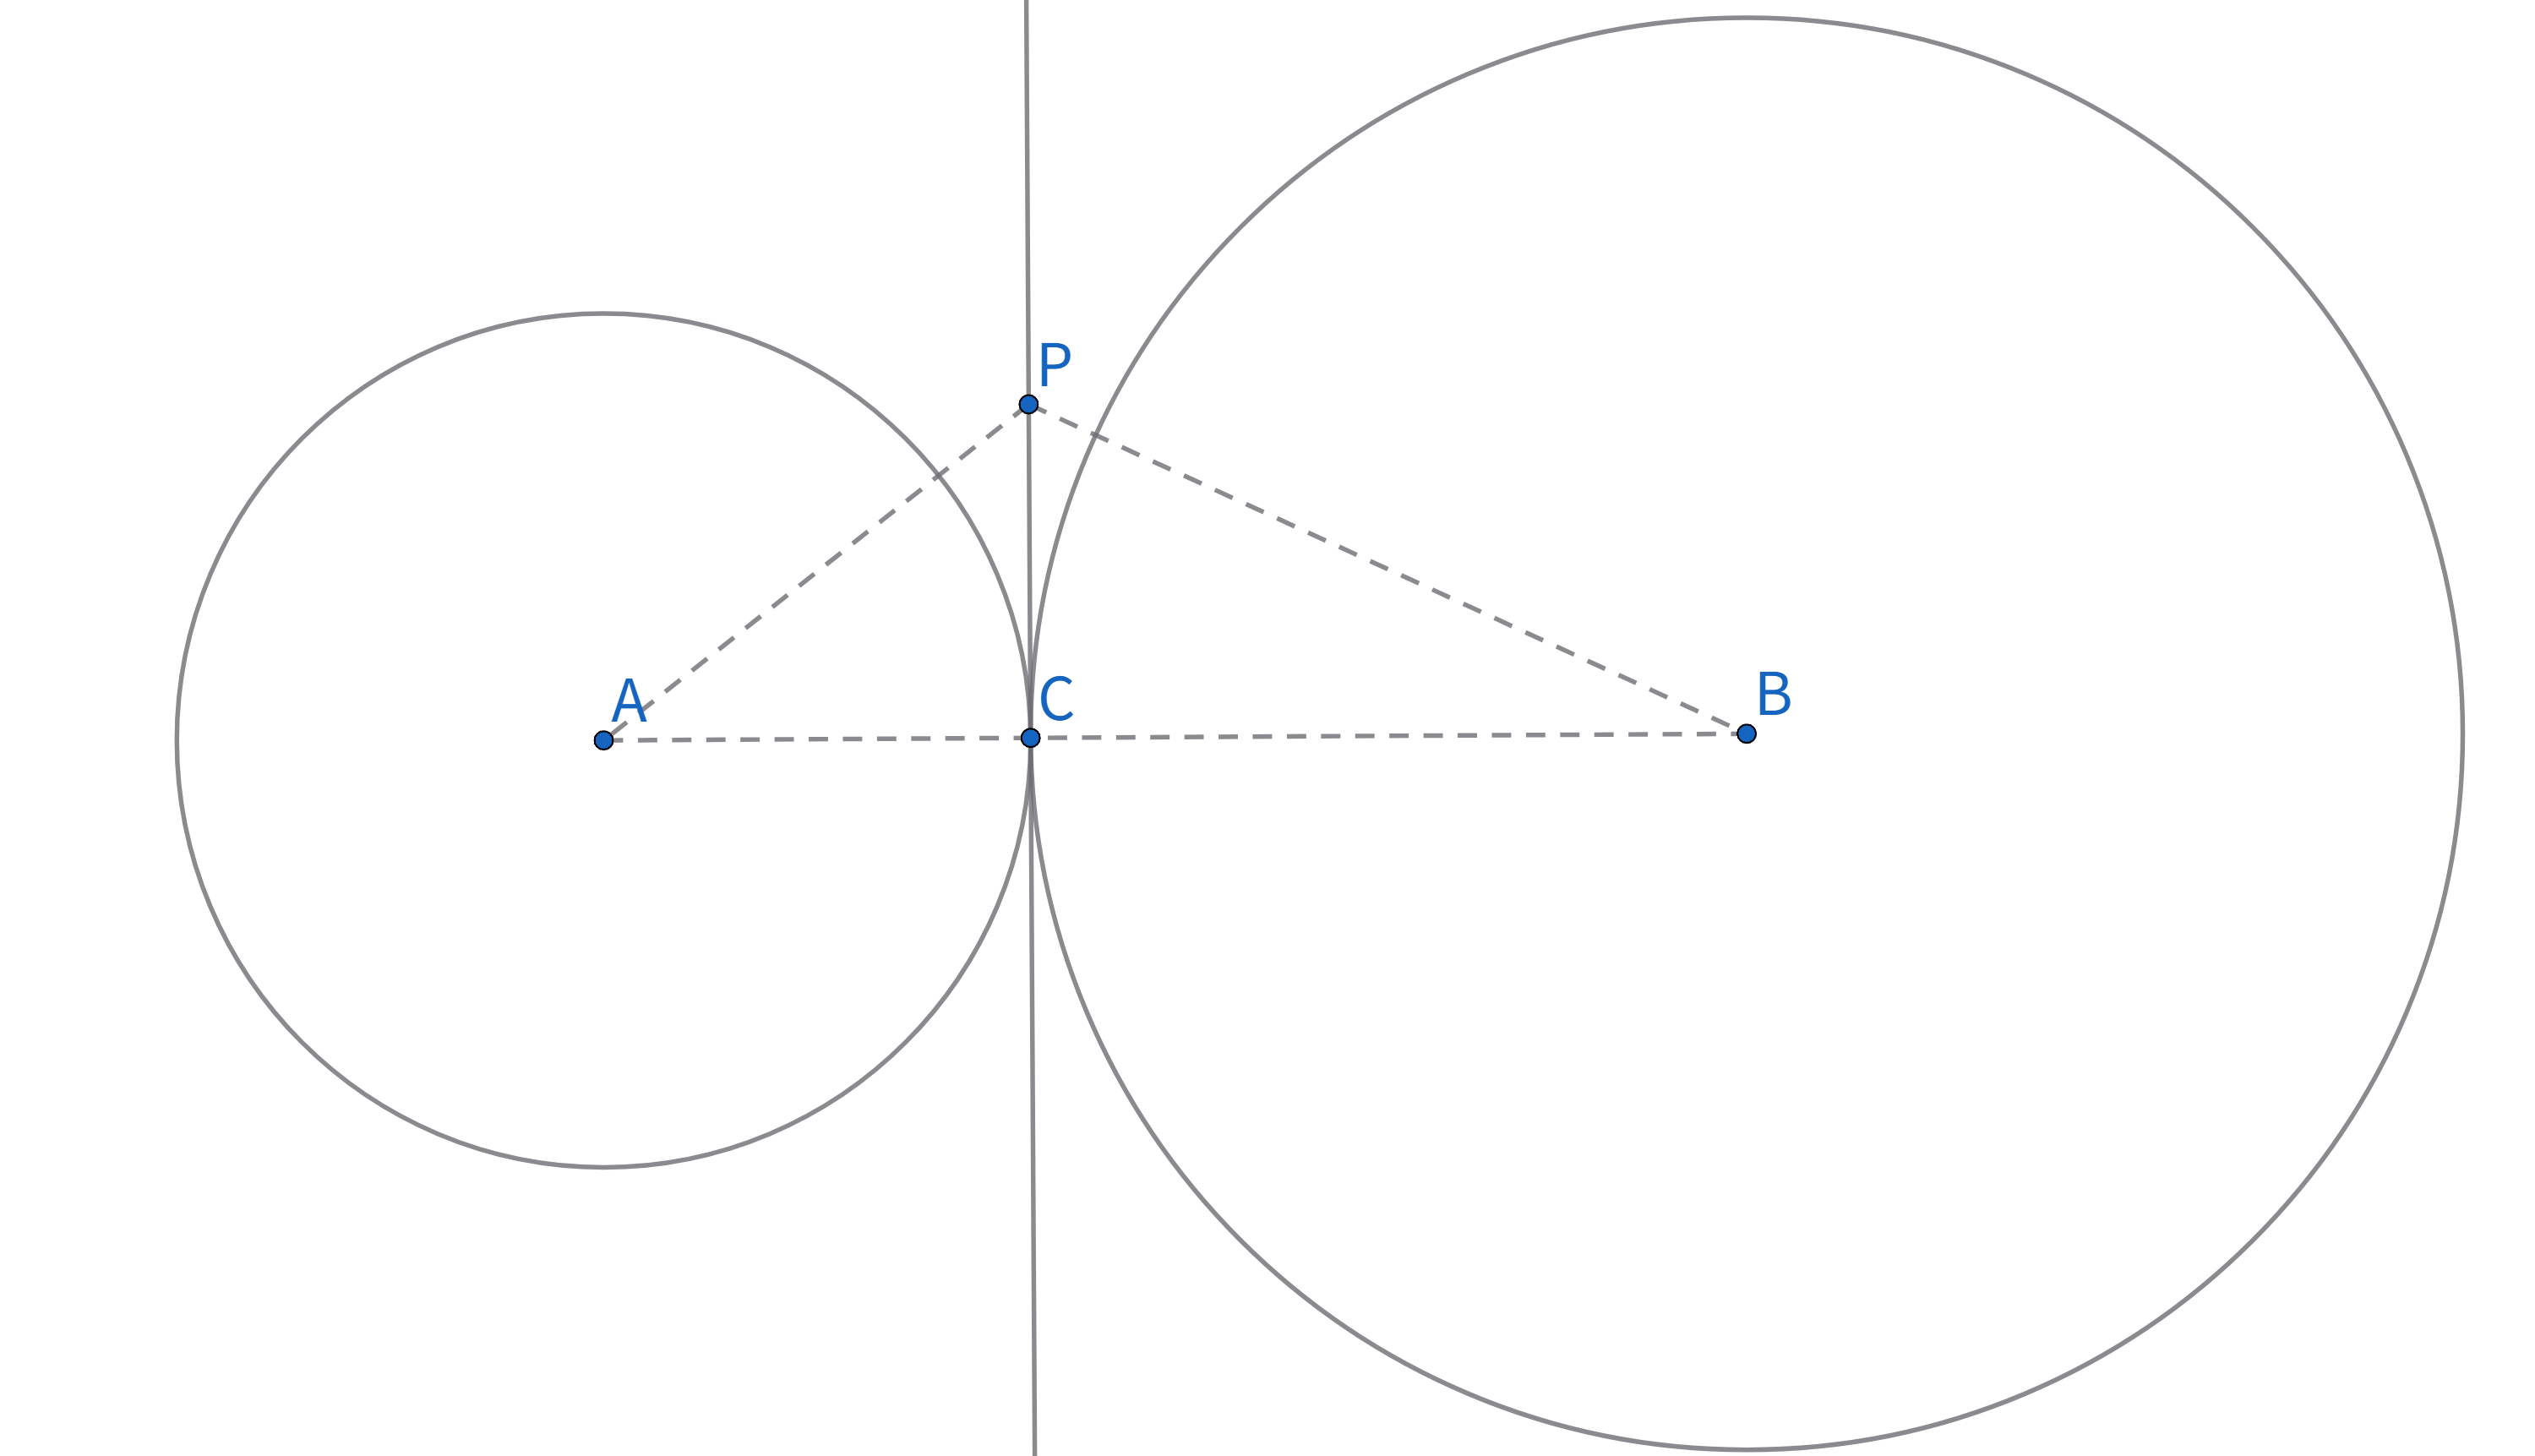
\includegraphics[width=\linewidth]{figures/相切圆根轴.png}
    \caption{相切圆根轴}
    \end{minipage}
    \begin{minipage}[t]{0.3\textwidth}
    \centering
    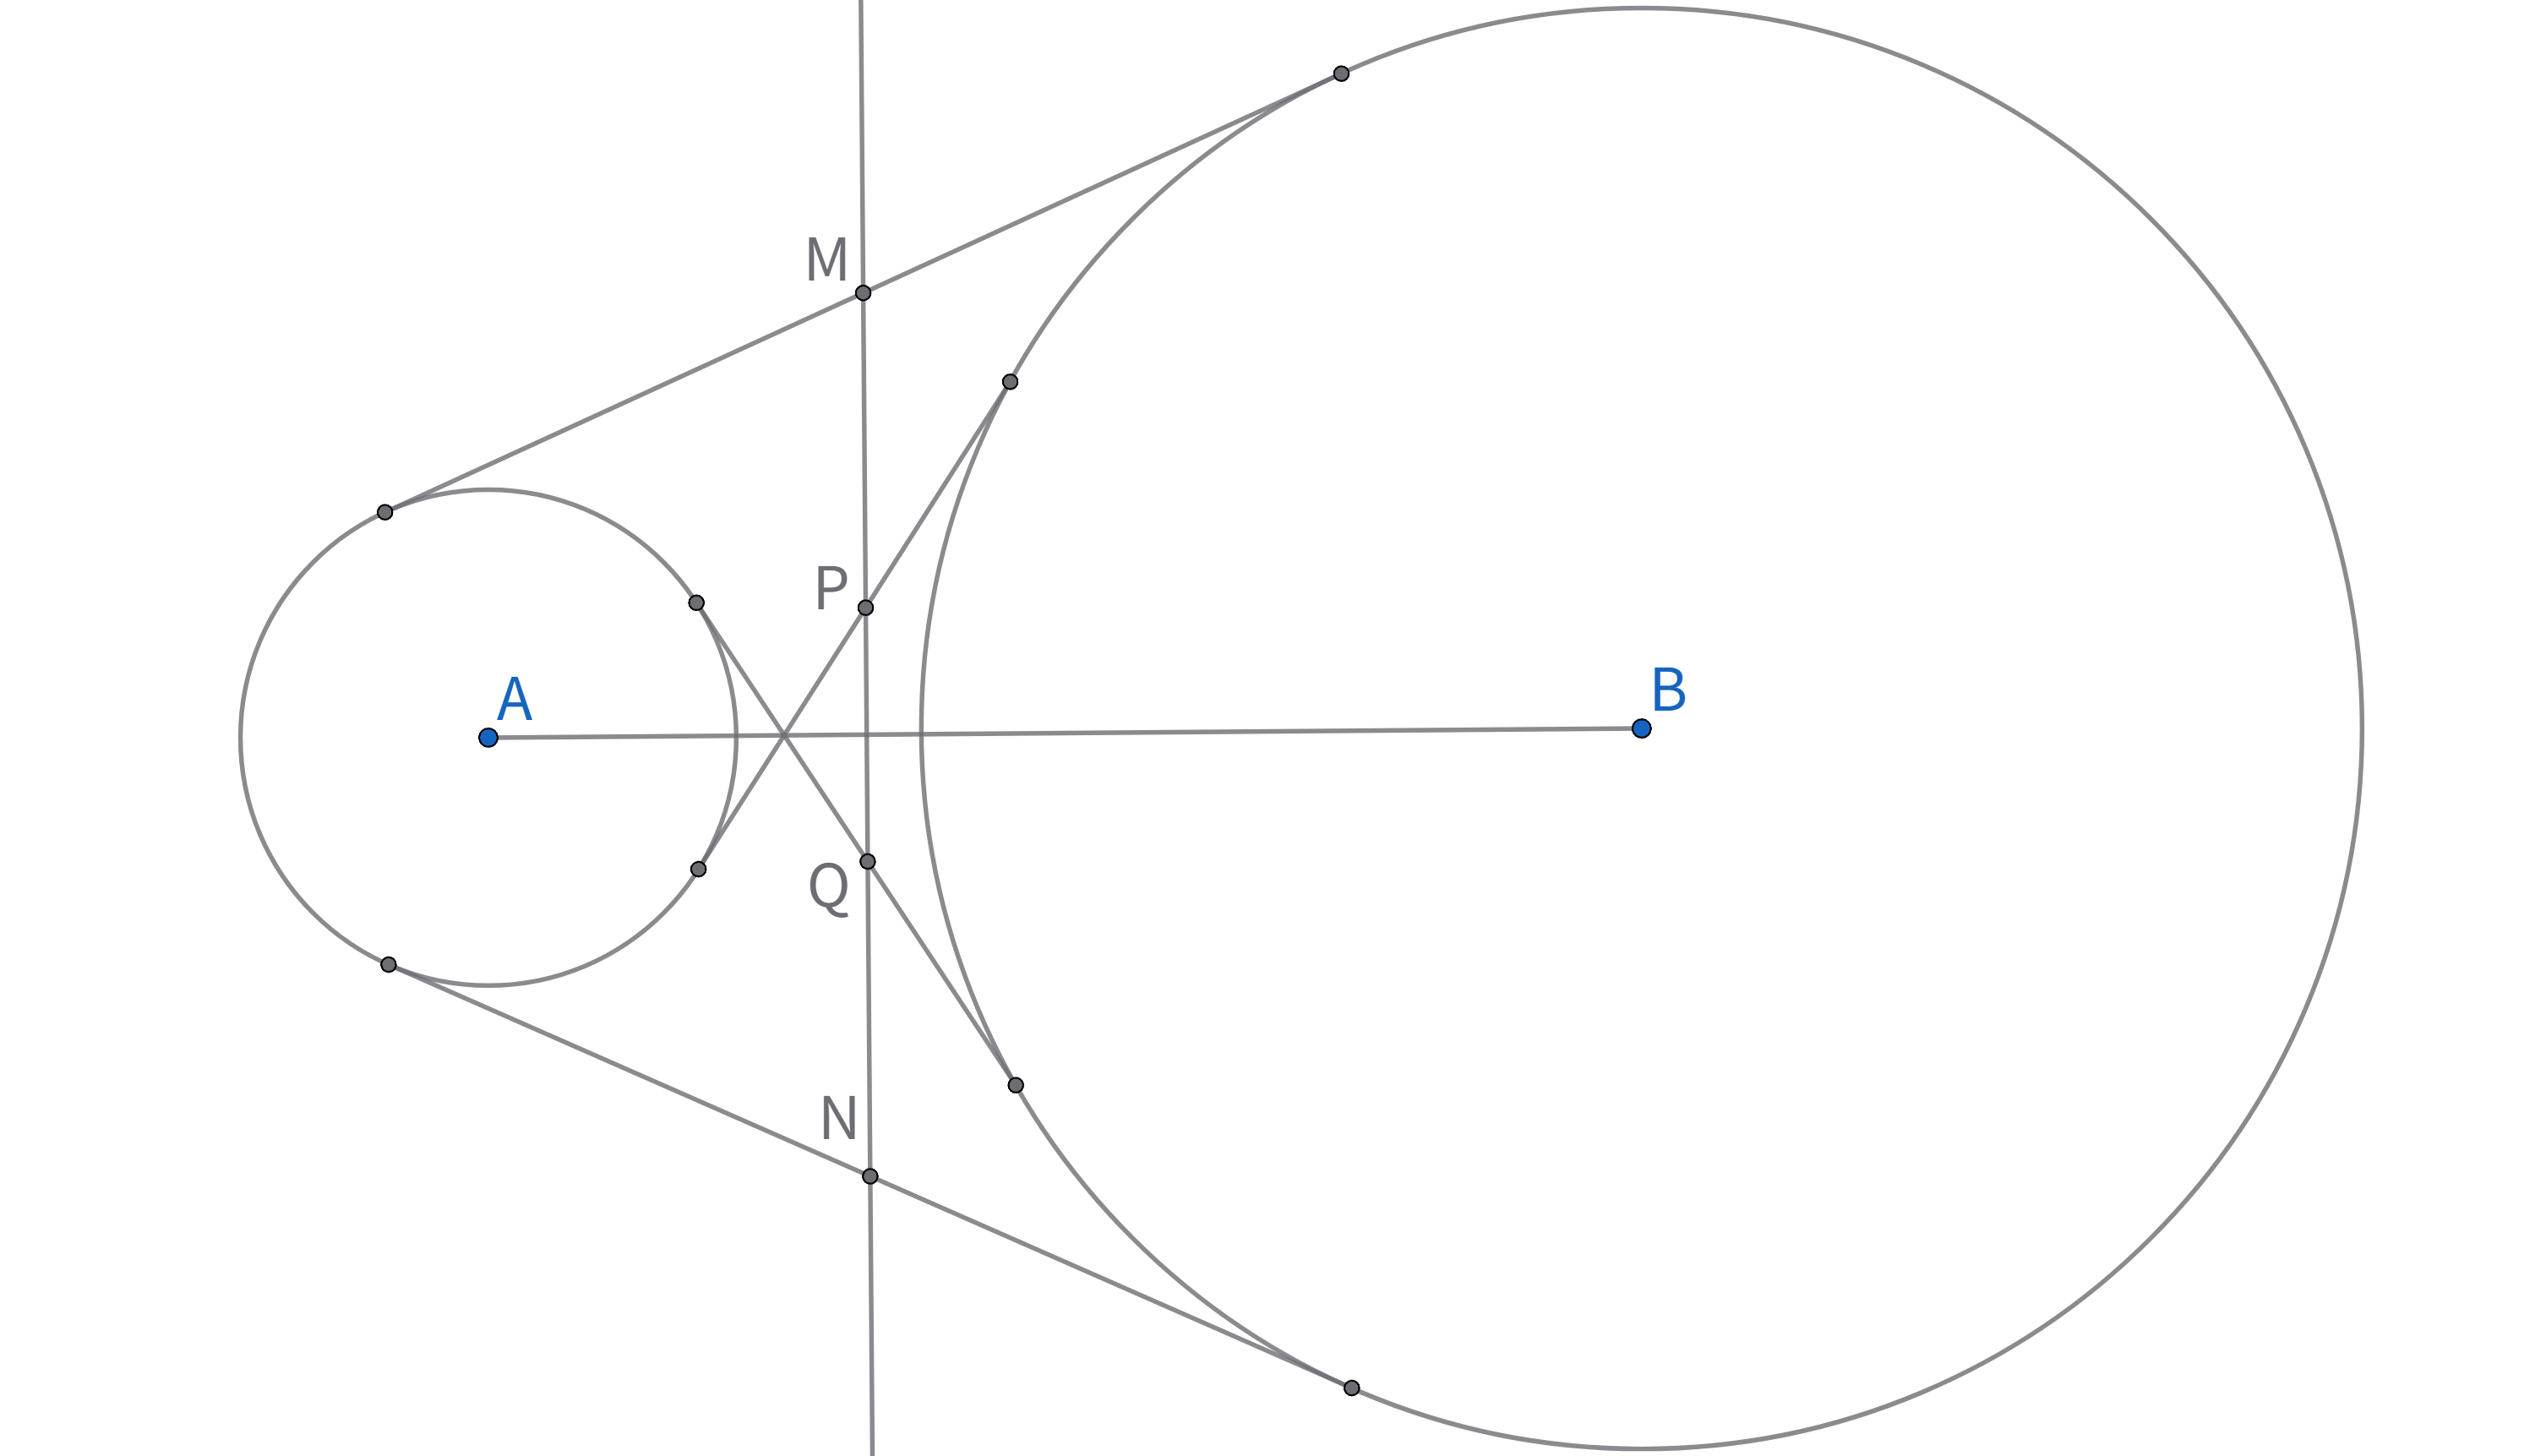
\includegraphics[width=\linewidth]{figures/相离圆根轴.png}
    \caption{相离圆根轴}
    \end{minipage}
\end{figure}


\begin{exercise}
    设 $P$ 在 $\triangle ABC$ 的内部,假设 $BC$ 与 $\triangle ABP$ 和 $\triangle ACP$ 的外接圆均相切。证明:射线 $AP$ 平分 $\overline{BC}$。
\end{exercise}

\begin{exercise}
    用根轴证明三角形的垂心存在,也就是说,若 $AD, BE, CF$ 是 $\triangle ABC$ 的三个高,证明它们共点。
\end{exercise}



%-------------------------------------------------------------
\newpage 
\section{根心}
\begin{theorem}[根心定理]
    平面内的三个定圆,他们两两的根轴或相交于一点,或互相平行。
\end{theorem}
\begin{figure}[H]
    \centering
    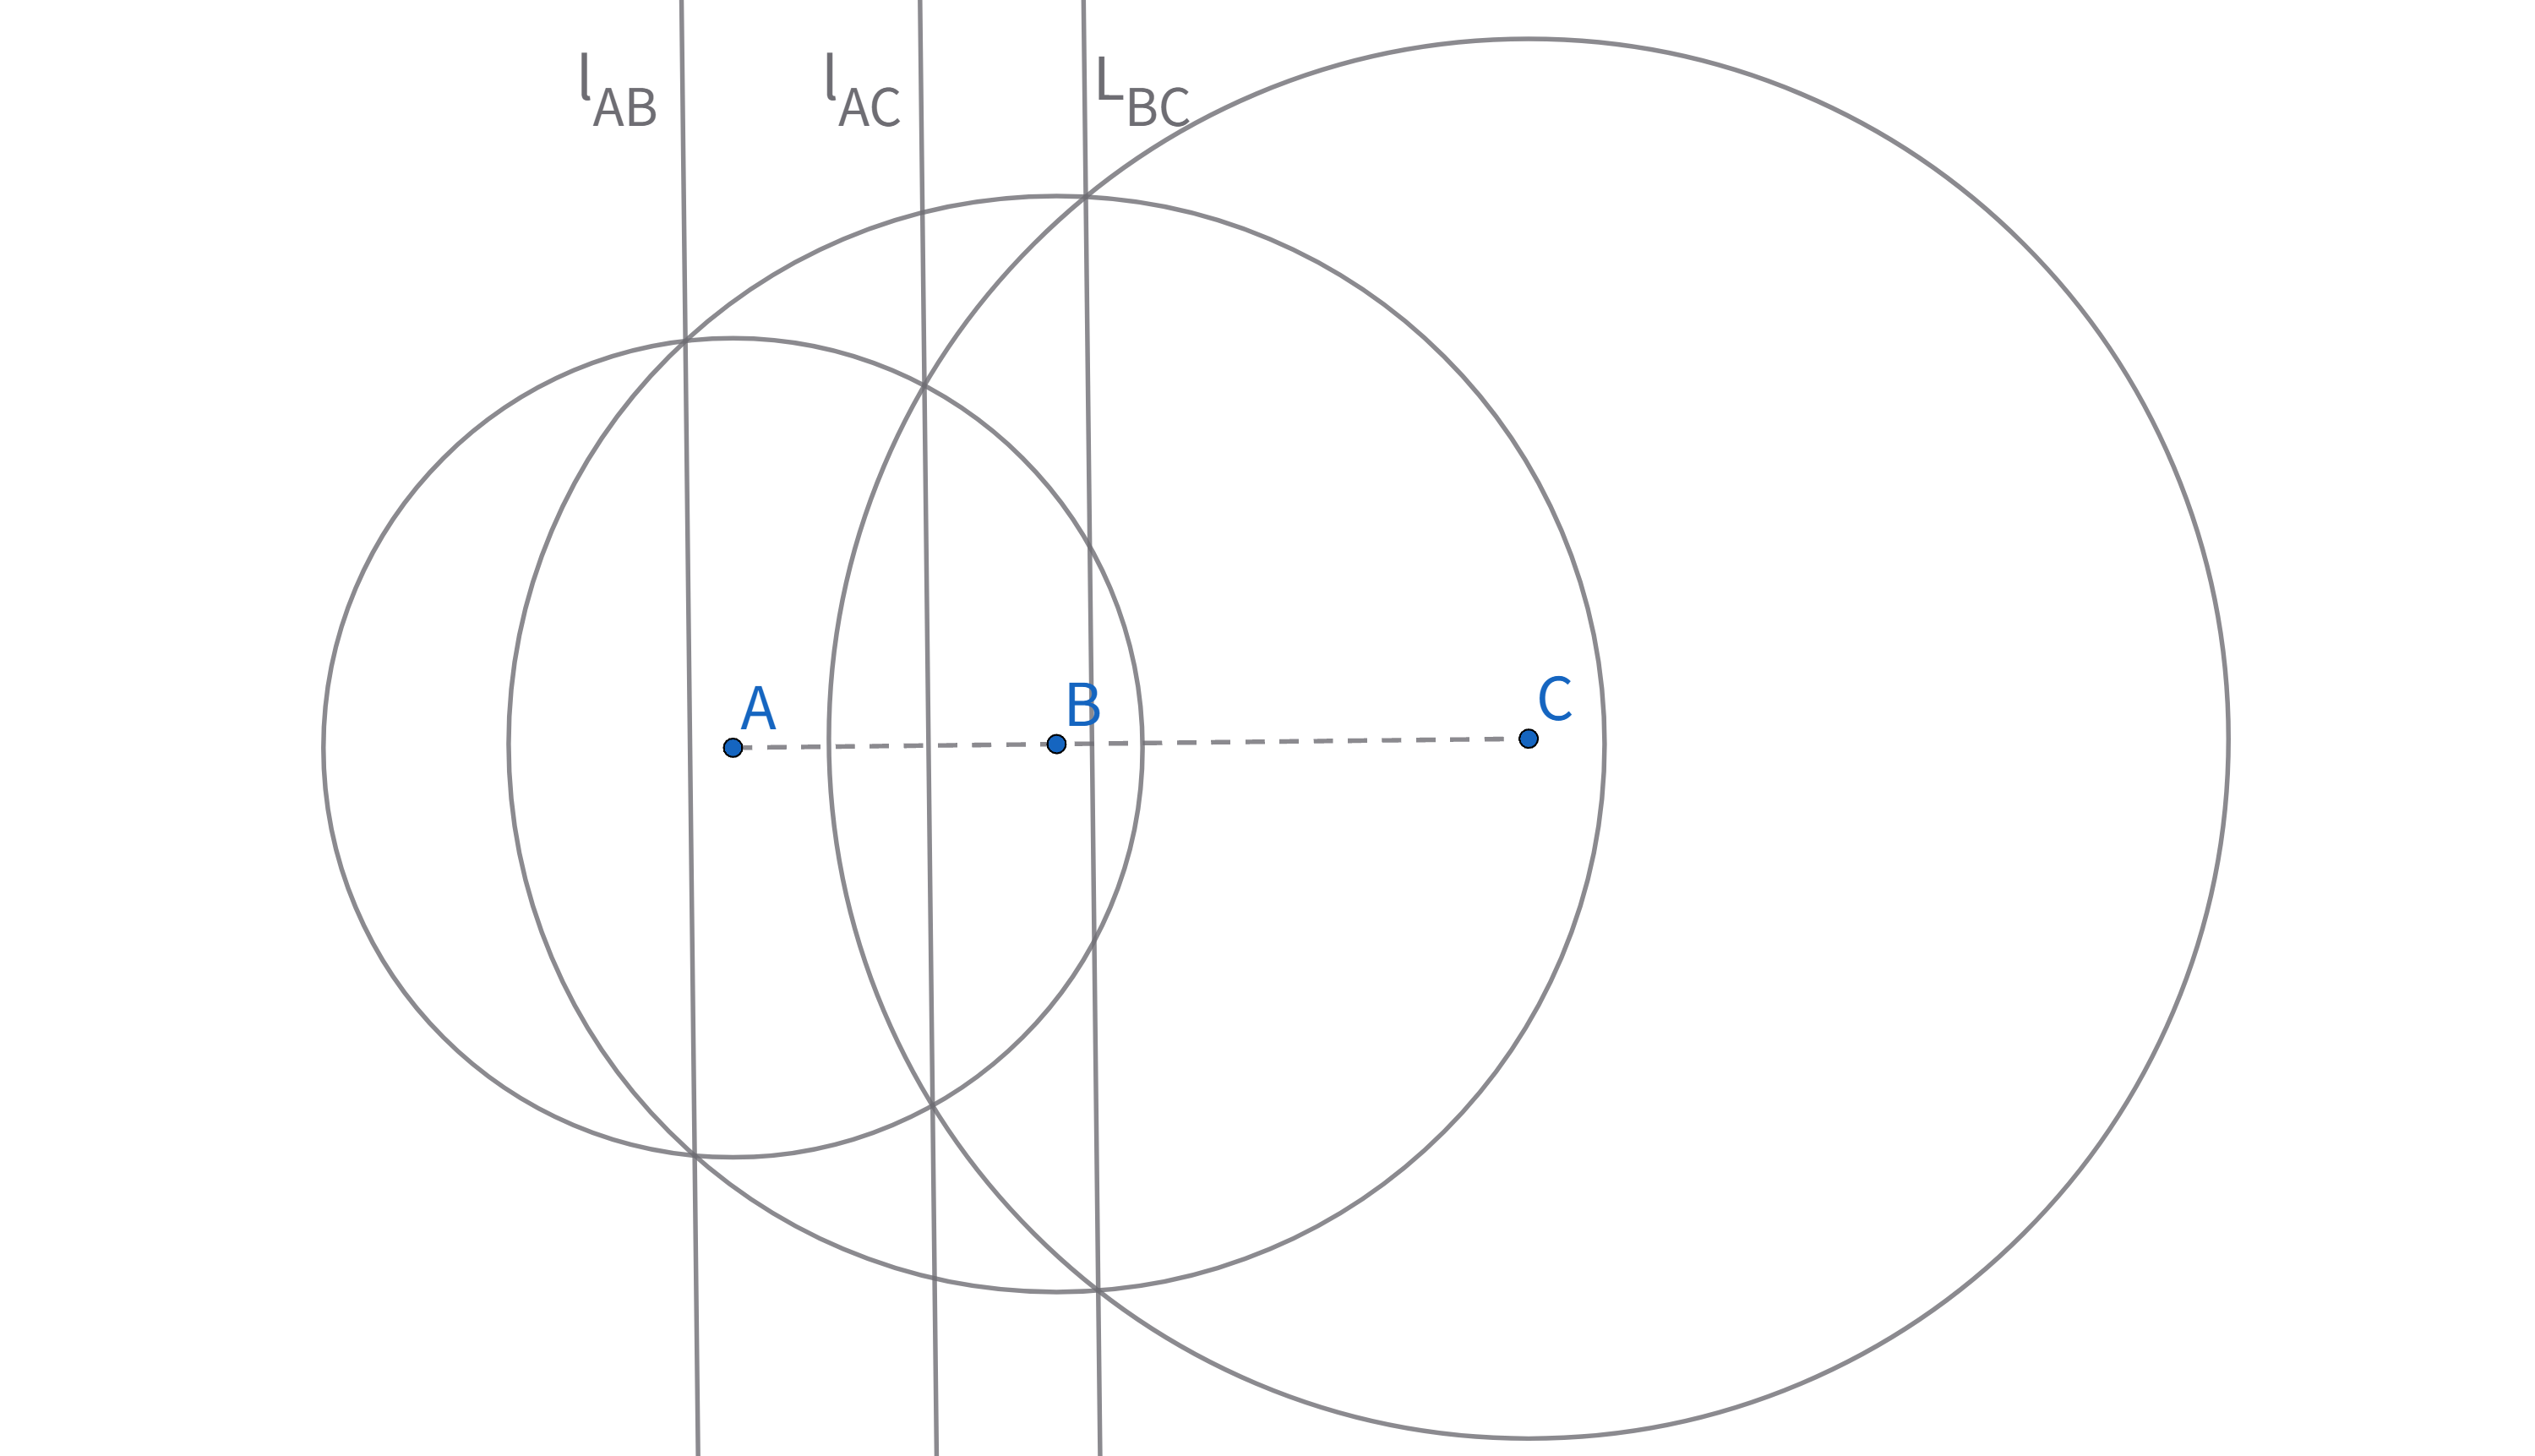
\includegraphics[width=0.8\linewidth]{figures/平行根轴.png}
    \caption{平行根轴}
\end{figure}
\begin{figure}[H]
    \centering
    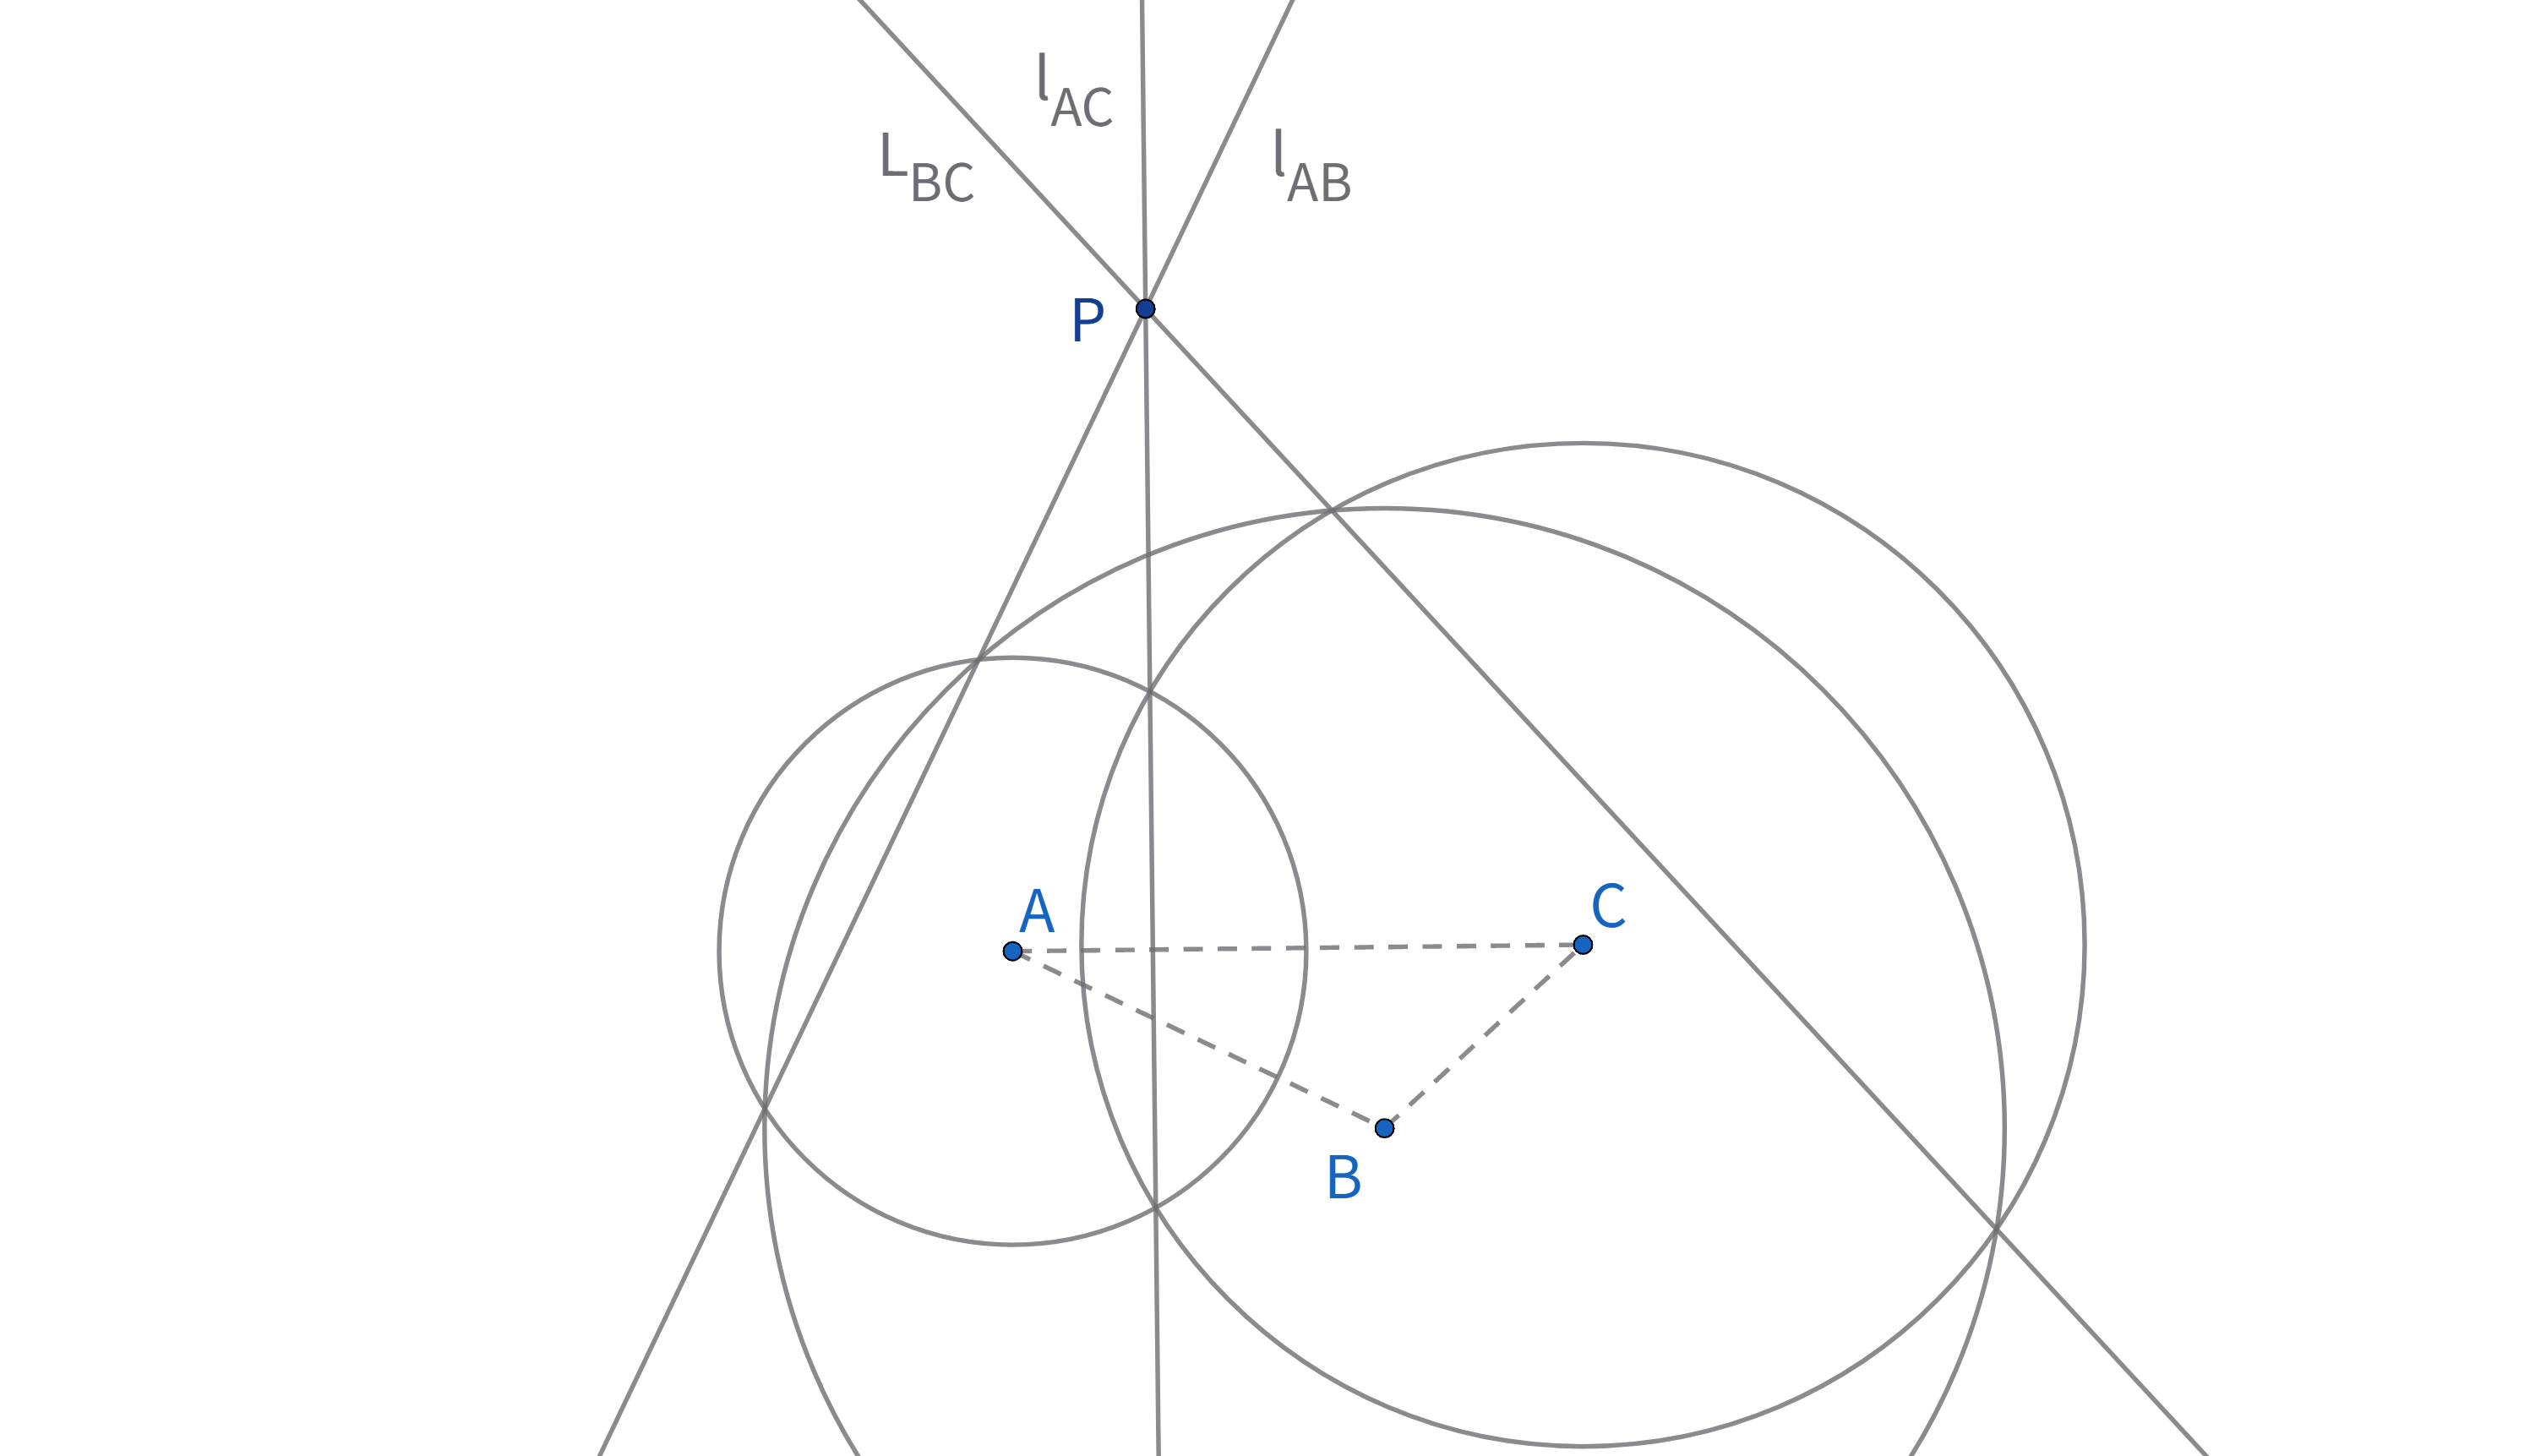
\includegraphics[width=0.8\linewidth]{figures/根心.png}
    \caption{根心}
\end{figure}